\documentclass{../Vorlage/sebDenCls}
\usepackage{graphicx}
\usepackage{caption}
\usepackage{subcaption}
\graphicspath{ {screenshots_documentation/} }

\begin{document}
\fach{Elektronische Bildverarbeitung}
\nr{1}
\abgabe{30.05.2017}
\semester{SoSe17}
\blatt{Udo Frese}{Lukas Bertram}{Sebastian Bliefert}{Johannes Hochbein}{Pascal Pieper}

\section{}
\subsection{Gesamtkonzept}
Um die Würfel im Versuchsaufbau zu zählen, wird das Eingabebild zunächst geeignet vorverarbeitet und anhand der Farben aufgeteilt. Die resultierenden Einzelbilder für jede Farbe werden binarisiert und anschließend einzeln der Würfelerkennung zugeführt. Diese ermittelt annähernd die geometrischen Mittelpunkte der segmentierten (Würfel-)flächen und nutzt diese Informationen zur Trennung der einzelnen Würfel mithilfe des \glqq watershed\grqq-Algorithmus. Anschließend werden die innerhalb der separierten Würfelflächen vorhandenen Augen mithilfe eines \glqq blob detectors\grqq  gezählt und in der Statistik der Augenverteilung erfasst.

\subsection{Teilalgorithmen}

\subsubsection{void preprocessColors(Mat\&img, double highestValue))}
\begin{itemize}
	\item \textbf{Mat\& img:} Referenz auf das Eingabebild
	\item \textbf{double highestValue:} Maximalwert, den die Farben annehmen können
\end{itemize}
Diese Funktion macht eine Farbwertspreizung, sodass der gesamte Farbbereich abgedeckt wird um die Segmentierung anhand von Farbwerten zu vereinfachen.

\subsubsection{void seperateDiceColors(Mat\& image, Mat\& display, vector $<$Dice$>$\& dices)}
\begin{itemize}
	\item \textbf{Mat\& image:} Referenz auf das Eingabebild
	\item \textbf{Mat\& display}: Referenz auf das zur Anzeige verwendete Bild 
	\item \textbf{vector$<$Dice$>$\& dices}: Verweis auf den mit den gefundenen Würfeln zu füllenden Vektor
\end{itemize}
Die Funktion \emph{seperateDiceColors(...)} extrahiert die für die einzelnen Würfelfarben relevanten Pixel aus dem Eingabebild und ruft \emph{segmentAndRecognizeFromBinImage(...)} für jedes der Ergebnisbilder auf.
Für die Extraktion wird das Eingabebild zunächst in den HSV-Farbraum konvertiert und anschließend mithilfe der openCV Funktion \glqq inRange()\grqq  auf das für die einzelnen Würfelfarben relevante Spektrum begrenzt und binarisiert. 

\subsubsection{void segmentAndRecognizeFromBinImage(Mat\& image, vector$<$Dice$>$\& dices)}
\begin{itemize}
	\item \textbf{Mat\& image}: Referenz auf das binäre Eingabebild
	\item \textbf{vector$<$Dice$>$\& dices}: Referenz auf den, mit den gefundenen Würfeln zu füllenden, Vektor
\end{itemize}


\texttt{segmentAndRecognizeFromBinImage()} segmentiert einzelne Würfel aus dem Eingabebild. Dazu werden auf einer Arbeitskopie des Bildes zunächst die Würfelflächen vollständig mit Weiß aufgefüllt (Hierfür Hintergrund per \texttt{floodfill()}) auffüllen, Ergebnis invertieren und auf das Eingabebild addieren), sodass die schwarzen Augen von den Würfelflächen verschwinden (siehe Abb. \ref{BEISPIEL}). 

\begin{figure}[htp]
 \centering 	
 \begin{subfigure}{0.5\textwidth}
 	 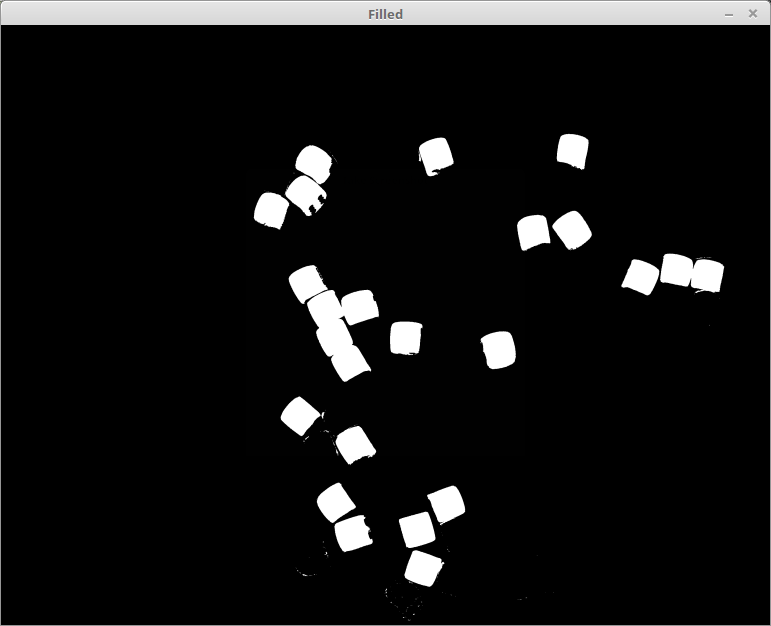
\includegraphics[width=.9\textwidth]{filled} 
 	 \caption{Filled image\label{BEISPIEL}}
 \end{subfigure}%
~
 \begin{subfigure}{0.5\textwidth}
 	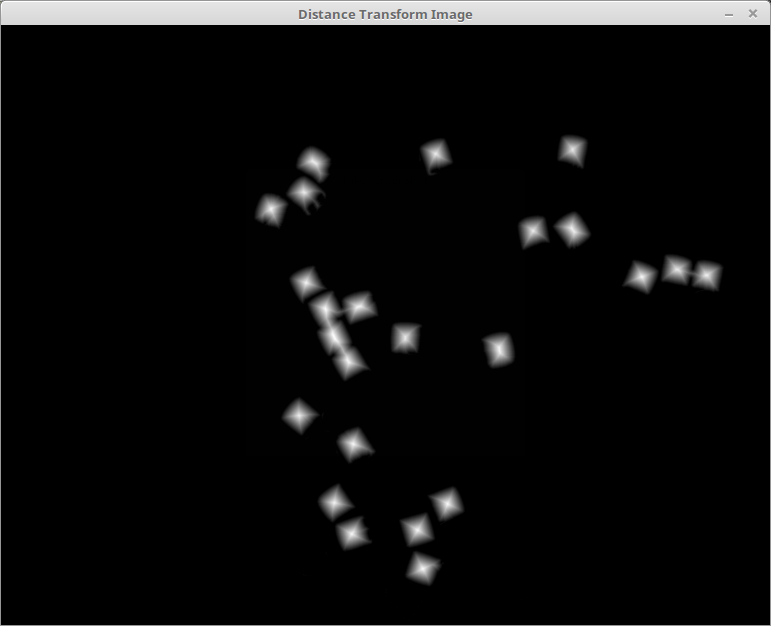
\includegraphics[width=.9\textwidth]{distanceTransform} 
 	\caption{Height map\label{distance}}
 \end{subfigure}\\
  \begin{subfigure}{0.5\textwidth}
  	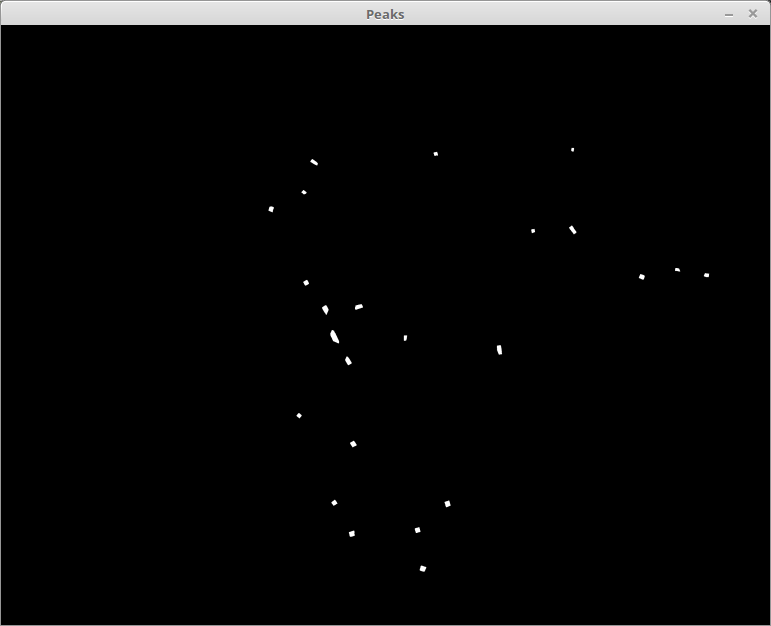
\includegraphics[width=.9\textwidth]{peaks} 
  	\caption{Peaks of height map\label{heightmap}}
  \end{subfigure}%
  ~
  \begin{subfigure}{0.5\textwidth}
  	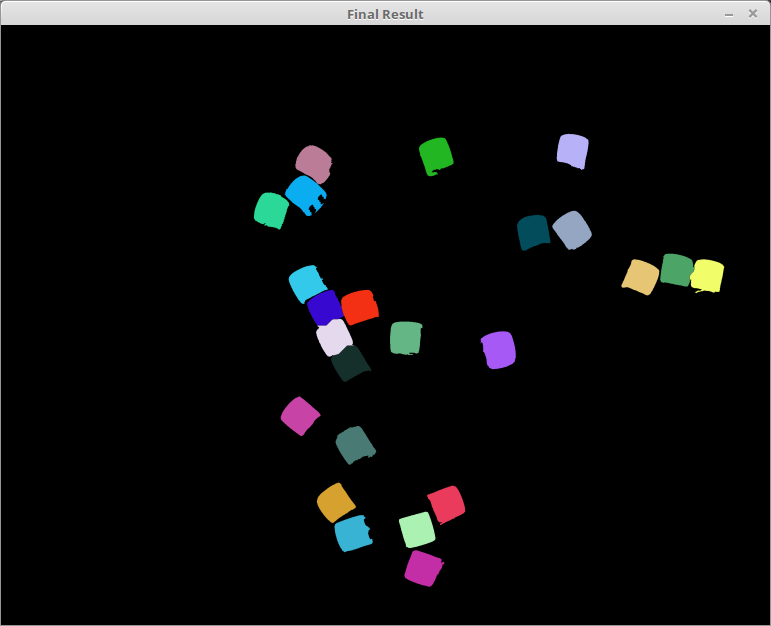
\includegraphics[width=.9\textwidth]{watershed} 
  	\caption{Coloration of watershed output\label{watershed}}
  \end{subfigure}\\

\begin{subfigure}{\textwidth}
	\centering
	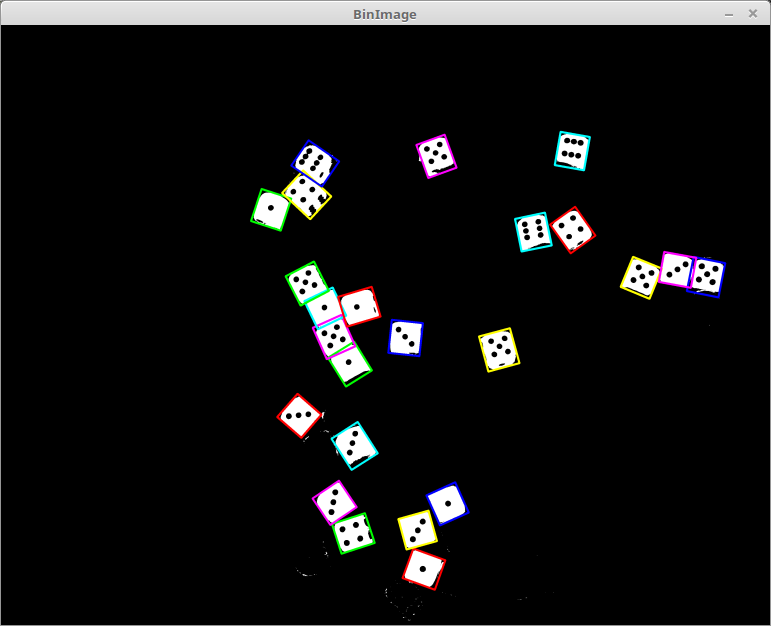
\includegraphics[width=.7\textwidth]{blobAreas} 
	\caption{Found Elems marked in original segmented image\label{result}}
\end{subfigure}\\
  \caption{Workflow of algorithm}
\end{figure}


Mithilfe dieses Bildes werden die \glqq Schwerpunkte\grqq  der Würfelflächen unter Verwendung des durch den distanceTransform-Algorithmus generierten Bilds (Abb. \ref{distance}) bestimmt: Das Ergebnisbild (8 Bit Graustufen) wird durch Anwendung eines Schwellwerts, Dilatation und anschließender Konturfindung überführt in einen Vektor aus Markern, die die \glqq Schwerpunkte\grqq  der Würfel repräsentieren. Mit \glqq Schwerpunkt\grqq  ist hier das Maximum der Entfernungen eines jeden Pixels innerhalb der Würfelfläche zum Rand der Fläche gemeint. 
Die so gewonnen Marker )Abb.  werden als Startpunkte für den Watershed-Algorithmus gebraucht, welcher die eigentliche Segmentierung der einzelnen Würfel vornimmt. Dazu füllt der Algorithmus das Eingabebild anhand der Marker in alle Richtungen auf, bis sich die einzelnen Füllgebiete entweder treffen oder der Hintergrund den Füllvorgang begrenzt (genauere Informationen zu \texttt{watershed(...)} unter \cite{opCV15}) und stellt die Konturen der so gefundenen Gebiete zur Verfügung (siehe Abb. \ref{watershed}). 
Aus jeder dieser Konturen wird mit\texttt{ minAreaRect(...)} das für die Augenzählung relevante Gebiet bestimmt und zusammen mit weiteren Parametern an \emph{countBlobs(...)} übergeben (siehe Abb. \ref{result}). Zusätzlich wird jeder gefundene Würfel im Vektor \emph{dices} für spätere Operationen abgelegt.

\subsubsection{Dice countBlobs(SimpleBlobDetector\& d, Mat\& orig, RotatedRect\& elem, vector$<$Point$>$\& approx)}
\begin{itemize}
	\item 
\end{itemize}
tbd

\subsubsection{void addToStatistics (vector$<$int$>$\& statistics, const vector$<$Dice$>$\& dices)}
\begin{itemize}
	\item 
\end{itemize}
tbd

\subsubsection{bool passed (const vector$<$int$>$\& statistics)}
\begin{itemize}
	\item 
\end{itemize}
tbd

\section*{Aufgabe 2}

tbd.

[CODE]

\section*{Aufgabe 3}

\subsection{Konzept:}
Der Keratograf sendet ein definiertes Muster aus konzentrischen, abwechselnd schwarzen und weißen Kreisen in Richtung Auge. Je nach Position des Auges vor dem Keratografen ergibt sich eine entsprechende Spiegelung der Ringe auf der Oberfläche der Hornhaut. Die Kamera ist im Zentrum des Keratografen platziert und nimmt das Bild der Spiegelung auf. Nach Bestimmung des gemeinsamen Mittelpunkts der Kreise wird der Abstand der Übergänge von Schwarz zu Weiß und von Weiß zu Schwarz entlang eines radialen Schnitts vermessen. Dazu wird eine Halbgerade festgelegt, die zunächst horizontal durch den Mittelpunkt verläuft und in diesem beginnt. Mit definierter Schrittweite wird der Schnittpunkt der Geraden mit einem fiktiven, zum Mittelpunkt konzentrischen Kreis auf diesem Kreis umlaufend verschoben. In jedem Zyklus werden nach einem "Weiterdrehen" alle Kanten in zur Halbgeraden senkrechter Richtung zunächst gefunden und dann in ihrem Abstand zum Mittelpunkt (Beginn der Halbgeraden und damit Urpsrung des zur Vermessung genutzten Koordinatensystems) vermessen. 

\subsection{Bewertung der Messwerte:}
Der theoretisch perfekte Abstand zwischen den Kanten ist bekannt für eine perfekt kugelfömige Honrhaut. Die Differenzen zwischen den theoretischen und den tatsächlich gemessenen Abständen gibt Aufschluss über die Form der Hornhaut: 
- Ist der gemessene Abstand kleiner als der theoretisch erwartete Wert, so ist die Hornhaut an dieser Stelle konkaver als die perfekte Kugel.
- Ist größer als der theoretisch erwartete Wert, so ist die Hornhaut an dieser Stelle konvexer als die perfekte Kugel.

\begin{thebibliography}{9}
	
	\bibitem{opCV15}
		OpenCV Documentation,
		\emph{Image Segmentation with Watershed Algorithm},
		\url{http://docs.opencv.org/3.1.0/d3/db4/tutorial_py_watershed.html},
		abgerufen am 30.05.17, 12:00Uhr.
	
\end{thebibliography}

\end{document}


